% Source PDF page 461 (printed p. 447)
\section*{习题}
\addcontentsline{toc}{section}{习题}
\subsection*{在集合上的投影}
\paragraph{8.1}\textit{投影的唯一性。}证明，若 $C\subseteq\R^n$ 非空、闭且凸，范数 $\norm{\cdot}$ 严格凸，则对每个 $x_0$，都恰好存在一个离它最近的 $x\in C$。换句话说，$x_0$ 在 $C$ 上的投影唯一。
\paragraph{8.2}[Web94, Val64] \textit{凸性的 Chebyshev 刻画。}若对每个 $x_0\in\R^n$，集合 $C\in\R^n$ 中都存在唯一离 $x_0$ 最近的点，距离采用欧氏范数，则称 $C$ 为 Chebyshev 集。根据习题8.1，每个非空闭凸集都是 Chebyshev 集。本题证明逆命题，即 Motzkin 定理。

设 $C\in\R^n$ 为 Chebyshev 集。
\begin{enumerate}[label=(\alph*)]
\item 证明 $C$ 非空且闭。
\item 证明在 $C$ 上的欧氏投影 $P_C$ 连续。
\item 设 $x_0\notin C$。证明，对所有 $x=\theta x_0+(1-\theta)P_C(x_0)$、$0\leq\theta\leq1$，有 $P_C(x)=P_C(x_0)$。
\item 设 $x_0\notin C$。证明，对所有 $x=\theta x_0+(1-\theta)P_C(x_0)$、$\theta\geq1$，有 $P_C(x)=P_C(x_0)$。
\item 合并(c)与(d)，可知以 $P_C(x_0)$ 为起点、方向为 $x_0-P_C(x_0)$ 的射线上，所有点的投影都是 $P_C(x_0)$。证明这意味着 $C$ 凸。
\end{enumerate}
\paragraph{8.3}\textit{在正常锥上的欧氏投影。}
\begin{enumerate}[label=(\alph*)]
\item \textit{非负正交象限。}证明在非负正交象限上的欧氏投影由原书第399页的表达式给出。
\item \textit{半正定锥。}证明在半正定锥上的欧氏投影由原书第399页的表达式给出。
\item \textit{二阶锥。}证明 $(x_0,t_0)$ 在二阶锥
\[K=\{(x,t)\in\R^{n+1}\mid\norm x_2\leq t\}\]
上的欧氏投影为
\[P_K(x_0,t_0)=\begin{cases}
0,&\norm{x_0}_2\leq-t_0,\\
(x_0,t_0),&\norm{x_0}_2\leq t_0,\\
\tfrac12(1+t_0/\norm{x_0}_2)(x_0,\norm{x_0}_2),&\norm{x_0}_2\geq|t_0|.
\end{cases}\]
\end{enumerate}
\paragraph{8.4}点在凸集上的欧氏投影，给出一个简单的分离超平面：
\[(P_C(x_0)-x_0)^\T\bigl(x-\tfrac12(x_0+P_C(x_0))\bigr)=0.\]
找出反例，说明这个构造对一般范数不成立。
\paragraph{8.5}[HUL93，第1卷，第154页] \textit{深度函数与到边界的有符号距离。}设 $C\subseteq\R^n$ 为非空凸集，$\dist(x,C)$ 为点 $x$ 在某范数下到 $C$ 的距离。已知 $\dist(x,C)$ 关于 $x$ 凸。
\begin{enumerate}[label=(\alph*)]
\item 证明深度函数
\[\operatorname{depth}(x,C)=\dist(x,\R^n\setminus C)\]
在 $x\in C$ 时凹。
\item 到 $C$ 边界的有符号距离定义为
\[s(x)=\begin{cases}\dist(x,C),&x\notin C,\\-\operatorname{depth}(x,C),&x\in C.\end{cases}\]
因此，$s(x)$ 在 $C$ 外为正，边界上为零，内部为负。证明 $s$ 为凸函数。
\end{enumerate}
% Source PDF page 462 (printed p. 448)
\subsection*{集合之间的距离}
\paragraph{8.6}设 $C,D$ 为凸集。
\begin{enumerate}[label=(\alph*)]
\item 证明 $\dist(C,x+D)$ 关于 $x$ 凸。
\item 证明 $\dist(tC,x+tD)$ 在 $t>0$ 时关于 $(x,t)$ 凸。
\end{enumerate}
\paragraph{8.7}\textit{椭球的分离。}设两个椭球定义为
\[\mathcal E_1=\{x\mid(x-x_1)^\T P_1^{-1}(x-x_1)\leq1\},\qquad
 \mathcal E_2=\{x\mid(x-x_2)^\T P_2^{-1}(x-x_2)\leq1\},\]
其中 $P_1,P_2\in\mathbb S_{++}^n$。证明，$\mathcal E_1\cap\mathcal E_2=\varnothing$ 当且仅当存在 $a\in\R^n$ 使
\[\norm{P_1^{1/2}a}_2+\norm{P_2^{1/2}a}_2<a^\T(x_1-x_2).\]
\paragraph{8.8}\textit{多面体的相交与包含。}设两个多面体定义为
\[P_1=\{x\mid Ax\preceq b\},\qquad P_2=\{x\mid Fx\preceq g\},\]
其中 $A\in\R^{m\times n}$、$b\in\R^m$、$F\in\R^{p\times n}$、$g\in\R^p$。说明如何通过求解一个或数量不多的 LP 可行性问题完成以下任务。
\begin{enumerate}[label=(\alph*)]
\item 找到交集 $P_1\cap P_2$ 中的一点。
\item 判断是否 $P_1\subseteq P_2$。
\end{enumerate}
对以下方式定义的两个多面体重复上述问题：
\[P_1=\conv\{v_1,\ldots,v_K\},\qquad P_2=\conv\{w_1,\ldots,w_L\},\]
其中 $v_1,\ldots,v_K,w_1,\ldots,w_L\in\R^n$。
\subsection*{欧氏距离与角度问题}
\paragraph{8.9}\textit{与给定数据最近的欧氏距离矩阵。}给定数据 $\widehat d_{ij}$、$i,j=1,\ldots,n$，它们是 $\R^k$ 中向量间欧氏距离受到干扰的测量值：
\[\widehat d_{ij}=\norm{x_i-x_j}_2+v_{ij},\qquad i,j=1,\ldots,n,\]
其中 $v_{ij}$ 为噪声或误差。对所有 $i,j$，数据满足 $\widehat d_{ij}\geq0$、$\widehat d_{ij}=\widehat d_{ji}$。维数 $k$ 未指定。

说明如何用凸优化求解：寻找维数 $k$ 及 $x_1,\ldots,x_n\in\R^k$，使 $\sum_{i,j=1}^n(d_{ij}-\widehat d_{ij})^2$ 最小，其中 $d_{ij}=\norm{x_i-x_j}_2$。换句话说，给定近似欧氏距离的数据，寻找最小二乘意义下最接近它们的一组真实欧氏距离。
\paragraph{8.10}\textit{极小极大角度拟合。}设 $y_1,\ldots,y_m\in\R^k$ 为变量 $x\in\R^n$ 的仿射函数：
\[y_i=A_ix+b_i,\qquad i=1,\ldots,m,\]
$z_1,\ldots,z_m\in\R^k$ 为给定非零向量。希望选择满足某些凸约束，例如线性不等式的 $x$，使 $y_i$ 与 $z_i$ 之间的最大夹角
\[\max\{\angle(y_1,z_1),\ldots,\angle(y_m,z_m)\}\]
最小。非零向量间角度按通常方式定义：
\[\angle(u,v)=\cos^{-1}\left(\frac{u^\T v}{\norm u_2\norm v_2}\right),\]
其中 $\cos^{-1}(a)\in[0,\pi]$。只关心最优目标值不超过 $\pi/2$ 的情况。

将此问题写成凸或拟凸优化问题。当 $x$ 的约束是线性不等式时，需要求解哪类问题？
% Source PDF page 463 (printed p. 449)
\paragraph{8.11}\textit{包含给定点的最小欧氏锥。}在 $\R^n$ 中，中心方向 $c\ne0$、角半径 $0\leq\theta\leq\pi/2$ 的欧氏锥定义为
\[\{x\in\R^n\mid\angle(c,x)\leq\theta\}.\]
欧氏锥是二阶锥，即能表示为二阶锥在非奇异线性映射下的像。

设 $a_1,\ldots,a_m\in\R^n$。怎样找到包含这些点、角半径最小的欧氏锥？特别地，应说明如何求解可行性问题，即判断是否存在包含这些点的欧氏锥。
\subsection*{极值体积椭球}
\paragraph{8.12}证明，内接于一个集合的最大体积椭球唯一。证明，一个集合的 Löwner--John 椭球唯一。
\paragraph{8.13}\textit{单纯形的 Löwner--John 椭球。}本题证明，$\R^n$ 中单纯形的 Löwner--John 椭球，必须缩小 $n$ 倍才能放入该单纯形内。由于 Löwner--John 椭球具有仿射不变性，只需对一个特定单纯形证明。

求单纯形 $C=\conv\{0,e_1,\ldots,e_n\}$ 的 Löwner--John 椭球 $\mathcal E_{\mathrm{lj}}$。证明，$\mathcal E_{\mathrm{lj}}$ 必须按因子 $1/n$ 缩小，才能放入单纯形内。
\paragraph{8.14}\textit{椭球内近似的效率。}设 $C$ 为 $\R^n$ 中多面体，$C=\{x\mid Ax\preceq b\}$，且 $\{x\mid Ax\prec b\}$ 非空。
\begin{enumerate}[label=(\alph*)]
\item 证明，内接于 $C$ 的最大体积椭球，围绕中心扩大 $n$ 倍后，得到包含 $C$ 的椭球。
\item 证明，若 $C$ 关于原点对称，即具有形式 $C=\{x\mid-\one\preceq Ax\preceq\one\}$，则将最大体积内接椭球扩大 $\sqrt n$ 倍，就得到包含 $C$ 的椭球。
\end{enumerate}
\paragraph{8.15}\textit{覆盖椭球并集的最小体积椭球。}将以下问题写成凸优化：寻找包含 $K$ 个给定椭球
\[\mathcal E_i=\{x\mid x^\T A_ix+2b_i^\T x+c_i\leq0\},\quad i=1,\ldots,K\]
的最小体积椭球 $\mathcal E=\{x\mid(x-x_0)^\T A^{-1}(x-x_0)\leq1\}$。
\textit{提示：}见附录B。
\paragraph{8.16}\textit{多面体内的最大体积矩形。}将以下问题写成凸优化：寻找位于多面体 $P=\{x\mid Ax\preceq b\}$ 内、体积最大的矩形
\[R=\{x\in\R^n\mid l\preceq x\preceq u\}.\]
变量为 $l,u\in\R^n$。所建模型不应包含指数数量的约束。
\subsection*{求中心}
\paragraph{8.17}\textit{解析中心的仿射不变性。}证明，不等式组的解析中心具有仿射不变性。证明，它在不等式正数缩放下保持不变。
\paragraph{8.18}\textit{解析中心与冗余不等式。}描述同一个多面体的两组线性不等式，可能具有不同解析中心。证明，通过加入冗余不等式，可以使多面体
\[P=\{x\in\R^n\mid Ax\preceq b\}\]
的任意内点 $x_0$ 成为解析中心。
% Source PDF page 464 (printed p. 450)
具体地，设 $A\in\R^{m\times n}$、$Ax_0\prec b$。证明，存在 $c\in\R^n$、$\gamma\in\R$ 以及正整数 $q$，使 $P$ 是如下 $m+q$ 个不等式的解集：
\begin{equation}Ax\preceq b,\qquad c^\T x\leq\gamma,\qquad c^\T x\leq\gamma,\quad\ldots,\quad c^\T x\leq\gamma,\tag{8.36}\end{equation}
其中不等式 $c^\T x\leq\gamma$ 添加 $q$ 次，并且 $x_0$ 是式(8.36)的解析中心。
\paragraph{8.19}设 $x_{\mathrm{ac}}$ 是线性不等式组
\[a_i^\T x\leq b_i,\qquad i=1,\ldots,m\]
的解析中心，定义 $H$ 为对数障碍在 $x_{\mathrm{ac}}$ 处的 Hessian：
\[H=\sum_{i=1}^m\frac1{(b_i-a_i^\T x_{\mathrm{ac}})^2}a_ia_i^\T.\]
证明，若
\[b_k-a_k^\T x_{\mathrm{ac}}\geq m(a_k^\T H^{-1}a_k)^{1/2},\]
则第 $k$ 条不等式冗余，即删去它不会改变可行集。
\paragraph{8.20}\textit{由线性矩阵不等式解析中心得到的椭球近似。}设 $C$ 为 LMI
\[x_1A_1+x_2A_2+\cdots+x_nA_n\preceq B\]
的解集，$A_i,B\in\mathbb S^m$，$x_{\mathrm{ac}}$ 为其解析中心。证明
\[\mathcal E_{\mathrm{inner}}\subseteq C\subseteq\mathcal E_{\mathrm{outer}},\]
其中
\[\mathcal E_{\mathrm{inner}}=\{x\mid(x-x_{\mathrm{ac}})^\T H(x-x_{\mathrm{ac}})\leq1\},\]
\[\mathcal E_{\mathrm{outer}}=\{x\mid(x-x_{\mathrm{ac}})^\T H(x-x_{\mathrm{ac}})\leq m(m-1)\},\]
$H$ 是对数障碍
\[-\log\det(B-x_1A_1-x_2A_2-\cdots-x_nA_n)\]
在 $x_{\mathrm{ac}}$ 处的 Hessian。
\paragraph{8.21}[BYT99] \textit{解析中心的最大似然解释。}采用原书第352页的线性测量模型
\[y=Ax+v,\]
其中 $A\in\R^{m\times n}$。假设噪声分量 $v_i$ 独立同分布，支撑为 $[-1,1]$。与测量 $y\in\R^m$ 一致的参数 $x$ 构成由线性不等式
\begin{equation}-\one+y\preceq Ax\preceq\one+y\tag{8.37}\end{equation}
定义的多面体。设 $v_i$ 的概率密度为
\[p(v)=\begin{cases}\alpha_r(1-v^2)^r,&-1\leq v\leq1,\\0,&\text{其他情况},\end{cases}\]
其中 $r\geq1$、$\alpha_r>0$。证明，$x$ 的最大似然估计为式(8.37)的解析中心。
\paragraph{8.22}\textit{重心。}内部非空的集合 $C\subseteq\R^n$ 的重心定义为
\[x_{\mathrm{cg}}=\frac{\int_C u\,du}{\int_C1\,du}.\]
% Source PDF page 465 (printed p. 451)
重心具有仿射不变性，而且显然取决于集合 $C$ 本身，而不是它的具体描述。不过，与本章介绍的其他中心不同，除椭球、球、单纯形等简单情况外，计算重心非常困难。

证明，重心 $x_{\mathrm{cg}}$ 是凸函数
\[f(x)=\int_C\norm{u-x}_2^2\,du\]
的最小点。
\subsection*{分类}
\paragraph{8.23}\textit{稳健线性判别。}考虑式(8.23)的稳健线性判别问题。
\begin{enumerate}[label=(\alph*)]
\item 证明，最优值 $t^\star$ 为正，当且仅当两组点可线性分离。在可线性分离时，证明最优 $a^\star$ 使 $\norm a_2\leq1$ 取等号，即 $\norm{a^\star}_2=1$。
\item 用换元 $\widetilde a=a/t$、$\widetilde b=b/t$ 证明问题(8.23)等价于 QP
\[\begin{array}{ll}
\text{最小化}&\norm{\widetilde a}_2\\
\text{约束为}&\widetilde a^\T x_i-\widetilde b\geq1,\quad i=1,\ldots,N,\\
&\widetilde a^\T y_i-\widetilde b\leq-1,\quad i=1,\ldots,M.
\end{array}\]
\end{enumerate}
\paragraph{8.24}\textit{对权重误差具有最大稳健性的线性判别。}给定 $\R^n$ 中可线性分离的两组点 $\{x_1,\ldots,x_N\}$、$\{y_1,\ldots,y_M\}$。8.6.1节介绍了怎样寻找既判别二者、又使函数值间隔最大的仿射函数。还可以考虑向量 $a$ 变化时的稳健性，$a$ 有时称为权重向量。给定使 $f(x)=a^\T x-b$ 分离两组点的 $a,b$，将权重误差裕量定义为使仿射函数 $(a+u)^\T x-b$ 不再分离两组点的最小 $u\in\R^n$ 的范数。换句话说，权重误差裕量为最大的 $\rho$，使
\[(a+u)^\T x_i\geq b,\quad i=1,\ldots,N,\qquad
 (a+u)^\T y_j\leq b,\quad i=1,\ldots,M\]
对所有 $\norm u_2\leq\rho$ 都成立。

说明如何在归一化约束 $\norm a_2\leq1$ 下，求使权重误差裕量最大的 $a,b$。
\paragraph{8.25}\textit{最接近球形的分离椭球。}给定两组向量 $x_1,\ldots,x_N\in\R^n$、$y_1,\ldots,y_M\in\R^n$，希望寻找偏心程度最小，即定义矩阵条件数最小，的椭球 $\mathcal E$，满足 $x_i\in\mathcal E$、$i=1,\ldots,N$，以及 $y_i\notin\operatorname{int}\mathcal E$、$i=1,\ldots,M$。将它写成凸优化问题。
\subsection*{布置与平面布局}
\paragraph{8.26}\textit{二次布置。}考虑 $\R^2$ 中由含 $N$ 个节点的无向图 $\mathcal A$ 定义的布置问题，代价为二次：
\[\text{最小化}\quad\sum_{(i,j)\in\mathcal A}\norm{x_i-x_j}_2^2.\]
变量为位置 $x_i\in\R^2$、$i=1,\ldots,M$；位置 $x_i$、$i=M+1,\ldots,N$ 已给定。定义 $u,v\in\R^M$ 为
\[u=(x_{11},x_{21},\ldots,x_{M1}),\qquad
 v=(x_{12},x_{22},\ldots,x_{M2}),\]
分别包含自由节点的第一、第二分量。
% Source PDF page 466 (printed p. 452)
证明，可通过求解两组线性方程
\[Cu=d_1,\qquad Cv=d_2\]
得到 $u,v$，其中 $C\in\mathbb S^M$。用图 $\mathcal A$ 给出 $C$ 的各系数的简单表达式。
\paragraph{8.27}\textit{带最小距离约束的问题。}考虑以 $x_1,\ldots,x_N\in\R^k$ 为变量的问题。目标 $f_0(x_1,\ldots,x_N)$ 凸，约束
\[f_i(x_1,\ldots,x_N)\leq0,\qquad i=1,\ldots,m\]
凸，即各 $f_i:\R^{Nk}\to\R$ 凸。此外有最小距离约束
\[\norm{x_i-x_j}_2\geq D_{\min},\quad i\ne j,\quad i,j=1,\ldots,N.\]
这一般是困难的非凸问题。

按照平面布局中的做法，可以构造凸的限制问题：它是凸问题，但可行集更小。求解限制问题容易，而且其任意解保证是原非凸问题的可行解。设 $a_{ij}\in\R^k$、$i<j$、$i,j=1,\ldots,N$ 满足 $\norm{a_{ij}}_2=1$。证明，限制问题
\[\begin{array}{ll}
\text{最小化}&f_0(x_1,\ldots,x_N)\\
\text{约束为}&f_i(x_1,\ldots,x_N)\leq0,\quad i=1,\ldots,m,\\
&a_{ij}^\T(x_i-x_j)\geq D_{\min},\quad i<j,\quad i,j=1,\ldots,N,
\end{array}\]
凸，并且任意可行点均满足最小距离约束。

\textit{注：}选择方向 $a_{ij}$ 有许多好的启发式方法。一种简单方法从近似解 $\widehat x_1,\ldots,\widehat x_N$ 出发，它不必满足最小距离约束，再取 $a_{ij}=(\widehat x_i-\widehat x_j)/\norm{\widehat x_i-\widehat x_j}_2$。
\subsection*{其他问题}
\paragraph{8.28}设两个多面体描述为
\[P_1=\{x\mid Ax\preceq b\},\qquad
 P_2=\{x\mid-\one\preceq Cx\preceq\one\},\]
其中 $A\in\R^{m\times n}$、$C\in\R^{p\times n}$、$b\in\R^m$。多面体 $P_2$ 关于原点对称。对 $t\geq0$、$x_c\in\R^n$，记
\[tP_2+x_c=\{tx+x_c\mid x\in P_2\},\]
即先将 $P_2$ 关于原点缩放 $t$ 倍，再将中心平移到 $x_c$ 后得到的多面体。

说明如何用一个 LP 或一组 LP 求解以下问题。
\begin{enumerate}[label=(\alph*)]
\item 寻找位于 $P_1$ 内的最大多面体 $tP_2+x_c$，即
\[\begin{array}{ll}\text{最大化}&t\\\text{约束为}&tP_2+x_c\subseteq P_1,\\&t\geq0.\end{array}\]
\item 寻找包含 $P_1$ 的最小多面体 $tP_2+x_c$，即
\[\begin{array}{ll}\text{最小化}&t\\\text{约束为}&P_1\subseteq tP_2+x_c,\\&t\geq0.\end{array}\]
\end{enumerate}
% Source PDF page 467 (printed p. 453)
两个问题的变量均为 $t\in\R$、$x_c\in\R^n$。
\paragraph{8.29}\textit{多面体外近似。}设 $P=\{x\in\R^n\mid Ax\preceq b\}$ 为多面体，$C\subseteq\R^n$ 为给定集合，不必凸。利用支撑函数 $S_C$，将以下问题写成 LP：
\[\begin{array}{ll}\text{最小化}&t\\\text{约束为}&C\subseteq tP+x,\\&t\geq0.\end{array}\]
这里 $tP+x=\{tu+x\mid u\in P\}$，是 $P$ 关于原点缩放 $t$ 倍再平移 $x$ 后的多面体。变量为 $t\in\R$、$x\in\R^n$。
\paragraph{8.30}\textit{分段圆弧曲线插值。}给定点列 $a_1,\ldots,a_n\in\R^2$。构造依次通过这些点的曲线，相邻两点间为圆弧，即圆的一部分，或线段，将线段视作半径无穷大的圆弧。有许多圆弧连接 $a_i,a_{i+1}$，用圆弧在 $a_i$ 处切线与线段 $[a_i,a_{i+1}]$ 的夹角 $\theta_i\in(-\pi,\pi)$ 参数化。因此，$\theta_i=0$ 意味着两点间圆弧实际上是线段；$\theta_i=\pi/2$ 意味着半圆，位于线段 $[a_1,a_2]$ 上方；$\theta_i=-\pi/2$ 意味着半圆，位于该线段下方。见下图。
\begin{center}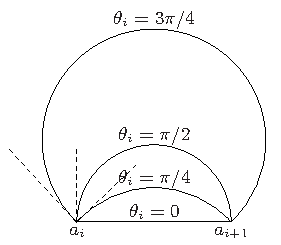
\includegraphics[width=.35\textwidth]{figures/ch08-ex467a.pdf}\end{center}
曲线由 $\theta_1,\ldots,\theta_n$ 完全指定，各角度可在 $(-\pi,\pi)$ 内选择。$\theta_i$ 的选择影响曲线的几种性质，例如总弧长 $L$，以及接点角不连续性，后者描述如下。

在每个 $a_i$、$i=2,\ldots,n-1$ 处，两段圆弧相接，一段从前一点而来，一段通向下一点。若两条切线方向恰好相反，从而曲线在 $a_i$ 处可微，则称该点没有接点角不连续。一般地，将 $a_i$ 处接点角不连续量定义为 $|\theta_{i-1}+\theta_i+\psi_i|$，其中 $\psi_i$ 为线段 $[a_i,a_{i+1}]$ 与 $[a_{i-1},a_i]$ 的夹角，即 $\psi_i=\angle(a_i-a_{i+1},a_{i-1}-a_i)$，如下图。由于各 $a_i$ 已知，角度 $\psi_i$ 也已知。
\begin{center}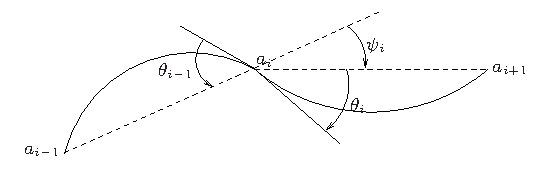
\includegraphics[width=.65\textwidth]{figures/ch08-ex467b.pdf}\end{center}
总接点角不连续量定义为
\[D=\sum_{i=2}^n|\theta_{i-1}+\theta_i+\psi_i|.\]
将最小化总弧长 $L$ 与总接点角不连续量 $D$ 的问题，写成双准则凸优化。说明如何找到最优权衡曲线上的极端点。
% Source PDF page 468 (printed p. 454): blank page in source.
